\section{Brownian motion}
Brownian motion was first observed by Robert Brown in 1827 \cite{Brown1828}, in these observations, Brown saw that microscopic particles (for example pollen grains) were in constant motion. He noticed that this motion was still present in inorganic material including granite and ground up Sphinx bones. 
\begin{quote}
To mention all the mineral substances in which I have found these molecules, would be tedious; and I shall confine myself in this summary to an enumeration of a few of the most remarkable. These were both of aqueous and igneous origin, as travertine, stalactites, lava, obsidian, pumice, volcanic ashes, and meteorites from various localities. Of metals I may mention manganese, nickel, plumhago, bismuth, antimony, and arsenic. In a word, in every mineral which I could reduce to a powder, sufficiently fine to be temporarily suspended in water, I found these molecules more or less copiously; and in some cases, more particularly in siliceous crystals, the whole body submitted to examination appeared to be composed of them. --\textbf{Robert Brown on what we now call Brownian particles}
\end{quote}
Over half a century later, Einstein showed that Brownian motion was due to constant bombardment by water molecules in the surrounding environment \cite{Einstein1905}, Einsteins theory of Brownian motion was then experimentally verified by Perrin \cite{Perrin2013}. The trajectory of a Brownian particle can either be described stochastically or with a probability distribution. Later work by Smoluchowski has allowed us to describe the evolution of the probability distribution of a Brownian particle mathematically using the Smoluchowksi equation which we will describe in section \ref{Smoluchowski}.

\section{Brownian motors}
Brownian motors are devices that can use stored energy to create directed motion on a microscopic scale. As well as being able to crank a rotor in the in the fashion of a traditional motor, they are also able to pump ions against a gradient and translocate molecules. Brownian motors have been implemented in the laboratory, for example Ref \cite{BlickleBechinger2011} created a stochastic heat engine by placing a single colloidal particle in a time dependent optical trap. Likewise, Ref \cite{Pedro2014} placed a colloidal particle in an optical tweezer and drove the particle with explosive vaporization of the surrounding liquid, thus demonstrating a thermal mechanism for Brownian motors. Brownian motors also include devices that can transport molecules over a long distance, for example Ref \cite{JoelBader1999} placed DNA molecules in a time dependent potential to transport the molecules. A very important class of Brownian motors are those where the energy is supplied by a chemical reaction. None of the above experiments fit this criteria, however these types of motors are ubiquitous in biology \cite{PhillipsQuakeMay2006, Magnasco1994}. Recently, thanks to improvements in imaging techniques, researchers have been able to make highly detailed images of these motors and their working components \cite{YiWeiChang2016}.

In this project, we will model Brownian motors using concepts from statistical mechanics. In particular, a Brownian motor will be modeled by a Brownian particle diffusing over its free energy landscape \cite{Reimann2001}, which in one dimension will be denoted by $x$. In the case of Brownian motion, it is natural to think of $x$ as a spatial coordinate, however in the case of Brownian motors this is not always the case. Often we will think of $x$ as a reaction coordinate for a chemical reaction, or in the case of a rotary motor, it could be the angle of the motor. We will think of a Brownian particle moving in titled periodic potential of the form $V(x) = f x + v_0(x)$ for some external forcing $f$ and some periodic function $v_0(x)$ with period $L$. This is shown schematically in figure \ref{fig:Schematic}, in this figure we have a particle with a certain known probability density. The particle is agitated by thermal vibrations in a random diffusive manner, however there is also a forcing on the particles that we describe using the potential. Different types of Brownian motors have been explored in the literature, including the Feynman ratchet \cite{Feynman1963}, the Landauer blowtorch \cite{Landauer1988}, thermal ratchets \cite{Pedro2014}, time dependent potentials \cite{JoelBader1999,BlickleBechinger2011} and tilted periodic potentials \cite{Leibler1993,Magnasco1994}.

\begin{figure}[tb]
	\centering
	\subfigure{%
		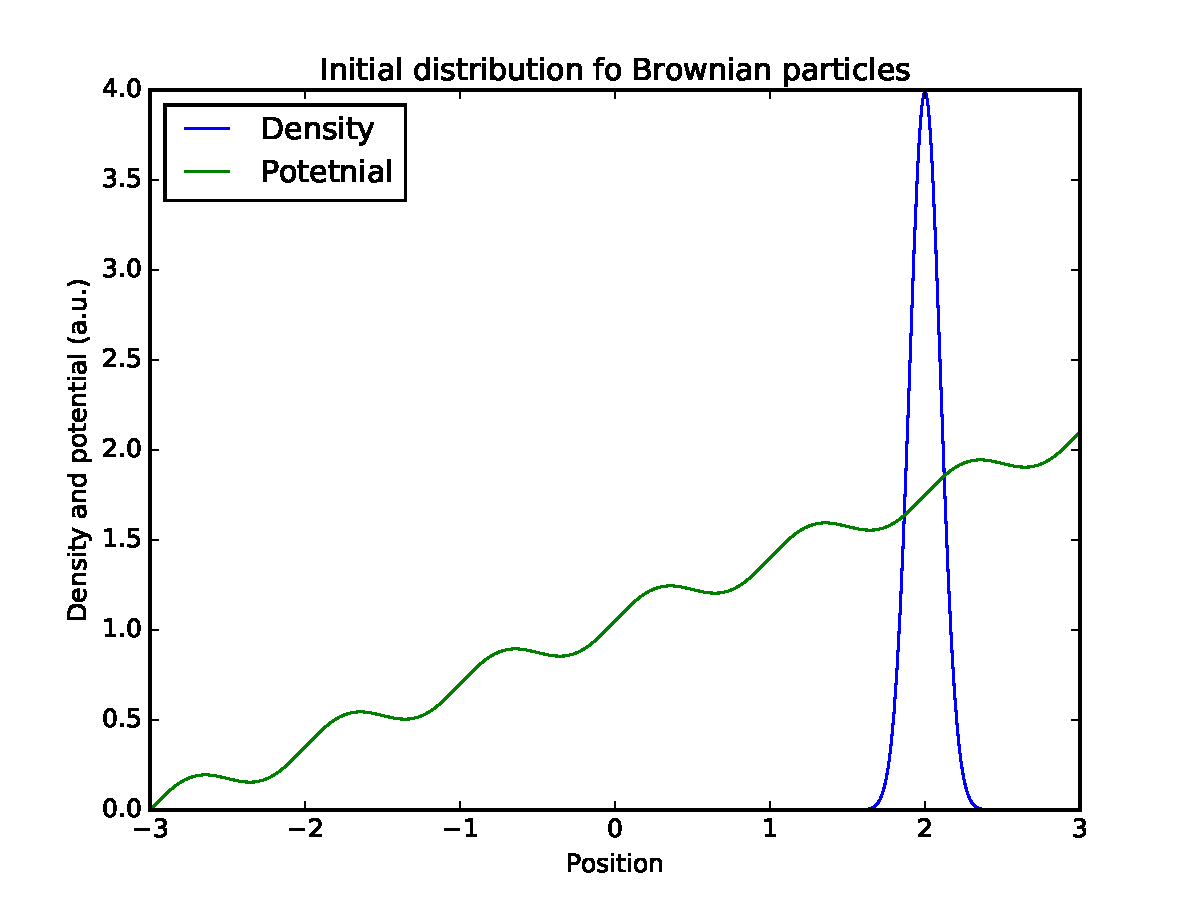
\includegraphics[width=0.45\columnwidth]{SchematicConstantTempInit}
	}
\quad
	\subfigure{
		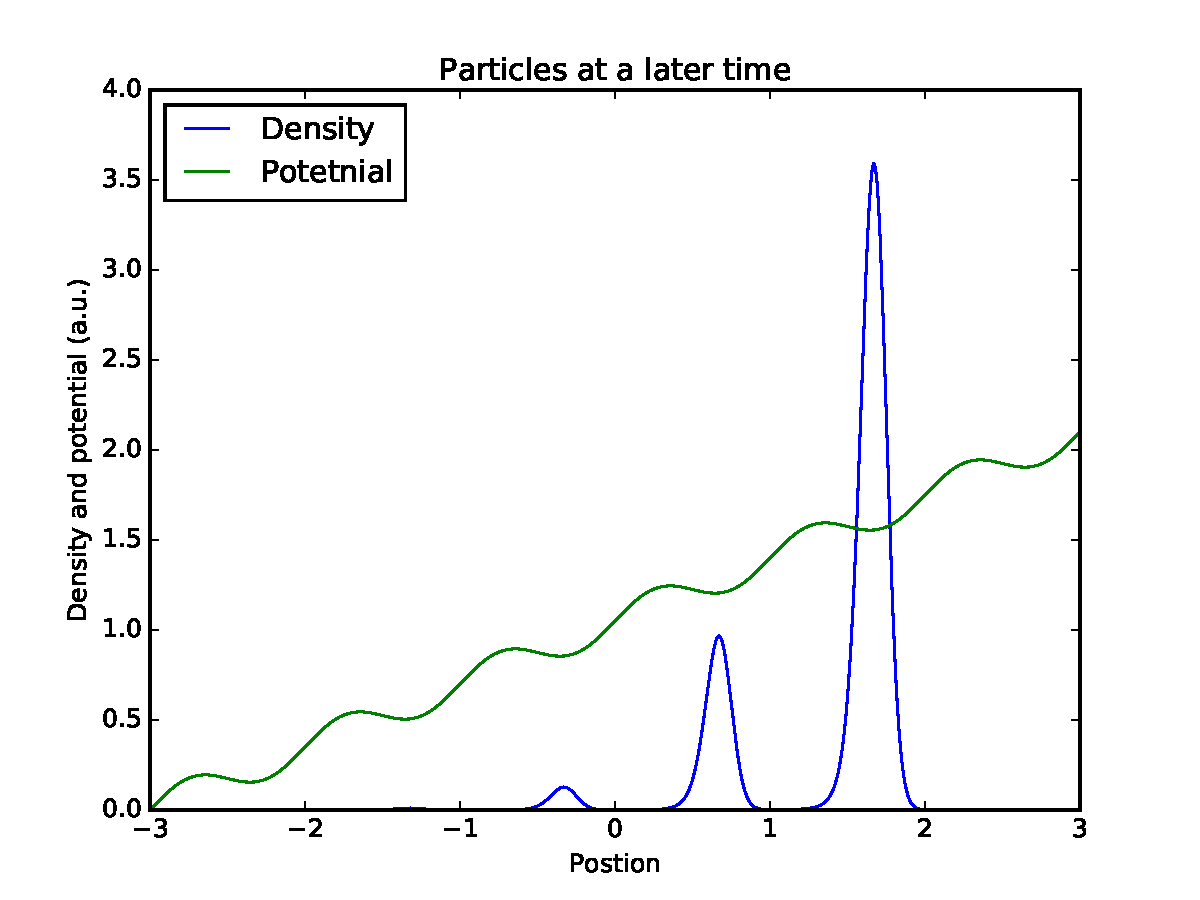
\includegraphics[width=0.45\columnwidth]{SchematicConstantTempFinal}
	}
\caption{Schematic showing the probability density of particles diffusing in a one dimensional tilted periodic potential at a fixed temperature. We see that the particles tend to drift down the potential as they diffuse, this drift will be called the current $J$ which we will quantify in section \ref{Smoluchowski}.}
\label{fig:Schematic}
\end{figure}

\section{Classes of Brownian motors} \label{BrownianMotorClasses}
Here we will discuss different classes of Brownian motors and their relationship to this project.

\subsection{Feynman ratchet and pawl}
The Feynman ratchet was initially discussed in the Feynman lectures \cite{Feynman1963} and was at first thought to be able to achieve greater than Carnot efficiency, however closer analysis showed that this was not possible \cite{ParrondoEspanol1996}. The system works as follows, we have two boxes that are thermally insulated from one another that are connected by an axle that can rotate. In one box there is a ratchet and pawl connected to the axle that makes it easy for the axle to turn one way (say clockwise), but hard to turn the other way (anti-clockwise). In the other box the axle is connected to paddles that are being buffeted by a gas (which we call the bath). The motion of the paddles are random since they are dictated by Brownian motion, so the purpose of the ratchet and pawl is to rectify the Brownian motion of these paddles. One may think that this could be used to do work (for example by using the axle to lift a weight), however this is not true. The problem is that the ratchet and pawl themselves will also be subject to random motion so they will sometimes allow the axle to turn anti-clockwise. To model the Feynman ratchet, we will need two degrees of freedom \cite{M.W.Jack2016}, this is beyond the scope of this project because we will only simulate systems with one degree of freedom.

\subsection{Landauer blowtorch}
The Landauer blowtorch scheme involves a temperature that varies in space \cite{Landauer1988}. As noted earlier, in order for the particles in Figure \ref{fig:Schematic} to get out of potential wells, they will need to acquire thermal energy from the environment. Landauer's idea was to assist these particles by heating the environment at the hills that the particles need to climb. From this Landauer notes that \cite{Landauer1988} ``The relative occupation of competing states of local stability is not determined solely by the characteristics of the locally favored states, but depends on the noise along the whole path connecting the competing states." This means that when we are modeling our system, we need to take non-constant temperatures into account.

\subsection{Thermal ratchet}
\cite{Pedro2014}

\subsection{Time dependent potentials}

\begin{figure}[tb]
	\centering
	\subfigure{%
		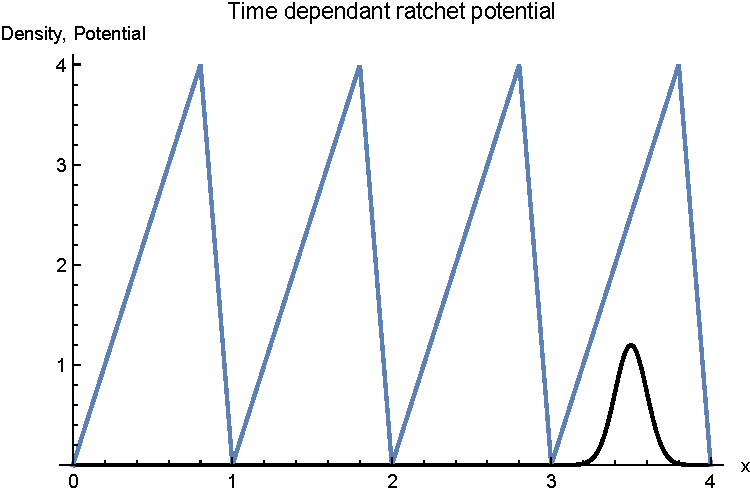
\includegraphics[width=0.45\columnwidth]{TimeDependentInit}
	}
\quad
	\subfigure{
		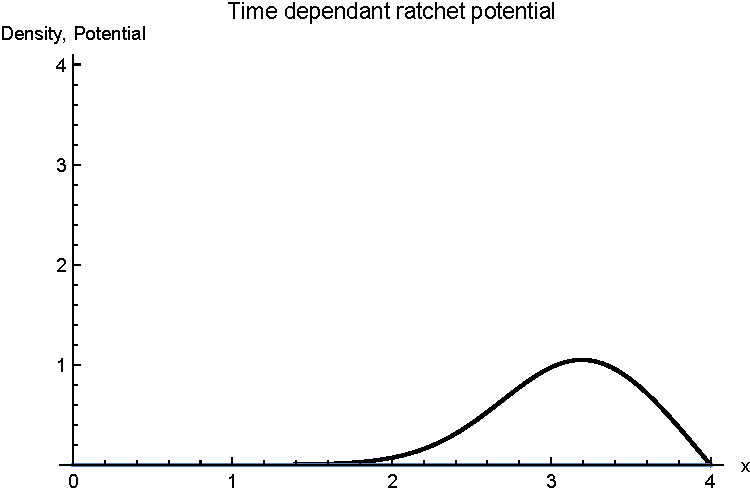
\includegraphics[width=0.45\columnwidth]{TimeDependentLater}
	}
	\subfigure{
		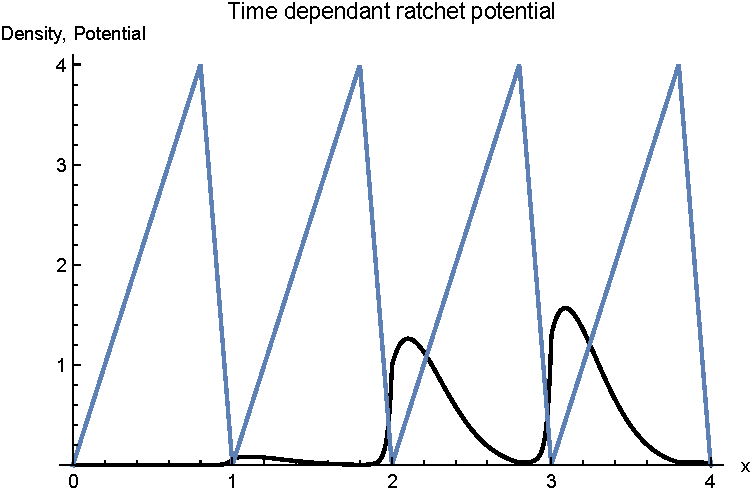
\includegraphics[width=0.45\columnwidth]{TimeDependentFinal}
	}
\caption{Schematic of particles diffusing in a time dependent potential, the blue line represents the potential and the black line represents the particle probability density. In (a) the particles are stuck in the first potential well, a certain time later the electric field is turned off and the particles diffuse freely as shown in part (b). When the potential is turned back on again, a large number of the particles will get stuck in the well to the left of the first one thus creating a net current to the left.}
\label{fig:TimeDependent}
\end{figure}

Both \cite{BlickleBechinger2011} \cite{JoelBader1999} are examples of experiments where a time dependent potential was used to do work on molecules. In \cite{JoelBader1999} DNA molecules are placed in a time dependent ratchet potential. When the electric field is on it creates a saw tooth shaped potential as shown in Figure \ref{fig:TimeDependent}, when the electric field is on, the molecules will go to the bottom of the wells and get stuck there. When the electric field is turned off however, the molecules will diffuse freely so that when the potential is turned back on at a later time, a large number of the molecules will then get trapped in the well to the left of where they were originally. Thus there is a net drift to the left.

\subsection{Tilted periodic potentials}
The tilted periodic potential (Figure \ref{fig:Schematic}) is of particular interest for this project because it can be used to model biological motors \cite{Leibler1993,Magnasco1994}. One way to model Brownian motors of this class is to think of a reaction coordinate $x$ that describes the conformation of a molecule in a chemical reaction. An example of this is the reaction ATP $\rightleftharpoons$ ADP + P, where ATP is adenosine tri-phosphate, ADP is adenosine di-phosphate and P is a lone phosphate molecule. This reaction coordinate is then coupled to a mechanical coordinate $y$ so that each time that a reaction takes place, the motor will move in some way. Since this is a chemical reaction, the free energy will be decreased as time moves forwards. So a system that has a potential that is periodic in $x$ is not sufficient to describe this situation, we will need to ``tilt" the potential by adding a forcing $f$. The value of $f$ will depend on the $\Delta G$ of the reaction (i.e. how far out of equilibrium the reaction is). It is shown in \cite{Magnasco1994} that this can be modeled by the two dimensional Smoluchowski equation. In this project we will only be modeling the one dimensional Somluchowski equation, so we will have to consider the case where $x$ and $y$ are tightly coupled. An example of tight coupling is the kinesin motor \cite{Leibler1993} that is used in cells to transport molecules. The kinesin motor is strongly bound to a track that it ``walks" along, on each step the motor will hydrolyze an ATP molecule using the reaction shown above. This reaction liberates about $12 k_B T$ Joules of energy that the motor uses to move forward. Kinesin motors are able to take many steps forward while taking few steps backwards all while falling off their track very infrequently \cite{BlockSM1990}.

\section{The Smoluchowski equation interacting with the environment} \label{Smoluchowski}

As we will see, the diffusion is increased by increasing the temperature and the drift is increased by increasing $f$. In some cases such as the Landauer blowtorch, the environment has a non uniform temperature held fixed by an external heat source \cite{Landauer1988}. With this in mind, we interpret Figure \ref{fig:Schematic} as follows: Brownian particles are subject to a given potential and are agitated by thermal noise, these agitations can give the particles the energy to move over barriers created by the potential. As one could imagine, these thermal interactions draw energy from the environment causing the temperature of the environment to change. Normally two simplifying assumptions are made at this point \cite{Reimann2001}, (i) that the thermal fluctuations created by the motor are very small compared to the thermal energy of the surrounding environment which is assumed to be effectively infinite, (ii) that when these temperature fluctuations occur, they diffuse away so rapidly that they do not need to be accounted for. In this project, we will question the second assumption in the case of Brownian motors. Assumption (ii) has also been questioned previously by Streater in the context of Brownian motion \cite{Streater1997, Streater1997a}. In these articles, Streater investigates Brownian motion from a microscopic view and then comes up with a mathematical model to describe Brownian particles that are thermally coupled to the environment, he then goes on to prove that the model is thermostatistically consistent in the sense that energy is conserved and that entropy increases. We will explore a similar set of equations in the context of Brownian motors and we will try to determine the length scales at which the thermal interaction is important.

This project will be focused on understanding the behavior of the coupled partial differential equations given by:

\begin{eqnarray}
J(x, t) &=& -\gamma^{-1} \frac{\partial}{\partial x} \left ( \frac{\partial V(x, t)}{\partial x} P(x, t) + k_B \frac{\partial}{\partial x} \left [T(x, t) P(x, t) \right] \right )  \\
\frac{\partial P(x, t)}{\partial t} &=& \frac{\partial J}{\partial x} \label{eqn:Smoluchowski} \\
\frac{\partial T(x, t)}{\partial t} &=& -\kappa q(x, t) + D \frac{\partial^2 T(x, t)}{\partial x^2} \label{eqn:TemperatureEvolution}
\end{eqnarray}

Where
\begin{itemize}
\item{$P(x, t)$ is the probability density as a function of  reaction coordinate $x$ and time $t$}
\item{$J(x, t)$ is called the current}
\item{$\gamma$ is the friction coefficient}
\item{$V(x, t)$ is the potential for the motor}
\item{$k_B$ is the Boltzmann constant}
\item{$q(x, t) = \partial_x V(x, t) J(x, t)$ is the heat from the motor}
\item{$\kappa$ is the thermal conductivity}
\item{$D$ is the thermal diffusivity}
\end{itemize}

Equation (\ref{eqn:Smoluchowski}) is called the Smoluschowski equation \cite{KellerBustamante2000} and equation \ref{eqn:TemperatureEvolution} is the heat equation. These equations make our intuitive notions more precise, we see that the first term on the right hand side of the Smoluchowski equation (equation \ref{eqn:Smoluchowski}) is a drift term that is forced by our potential and that the second term contains a diffusion term that is scaled by our temperature. In fact, Figure \ref{fig:Schematic} was made by solving equation (\ref{eqn:Smoluchowski}) numerically. Likewise, equation (\ref{eqn:TemperatureEvolution}) also appeals to how our intuition of how the motor should effect its environment. The first term represents the heat flux being produced by the motor \cite{M.W.Jack2016}, while the second term represents the diffusion of temperature into the environment.

% THERMODYNAMICS
\section{System thermodynamics}
The potential energy of the particle is $U_P = \int V(x) P(x) dx$ and the thermal energy of the environment is $c_p \int T(x) dx$, where $c_p$ is the specific heat capacity of the environment, with this we have.
\begin{equation}
E(t) = \int V(x)P(x, t) dx + c_p \int T(x, t) dx
\end{equation}
By using the Smoluchowski equation and the heat equation, we can differentiate with respect to time to get:
\begin{align}
\frac{d E}{d t} & = \int V(x) \frac{\partial P}{\partial t} dx + c_p \int \frac{\partial T}{\partial t} dx \\
 & = -\int V(x) \frac{\partial J}{\partial x} + c_p \int -\kappa J(x) \frac{\partial V}{\partial x} + D \frac{\partial^2 T}{\partial x^2} dx \\
 & = [V(x)J(x)]_{-\infty}^\infty + \int \frac{\partial V}{\partial x} J(x) dx - \kappa c_p \int \frac{\partial V}{\partial x} J(x) dx + D \left [\frac{\partial T}{\partial x} \right]_{-\infty}^{\infty}
\end{align}
If there are no particles are flowing through the boundaries and if there is no heat flowing through the boundaries, then there is no exchange of energy with the external environment. If we let $\kappa = \frac{1}{c_p}$, then the middle terms cancel and the first law is obeyed by the system.

As for the entropy, we have \cite{Streater1997a}
\begin{equation}
S(t) = -\int P(x, t) \log(P(x, t)) dx + c_p \int \log(T(x, t))dx
\end{equation}
Differentiating with respect to time, we get

\begin{align}
\frac{d S}{d t} =  \int \frac{\partial J}{\partial x} + \frac{\partial J}{\partial x} \log P \ dx + c \int \frac{1}{T} \left(-\kappa J \partial_x V + c \beta \frac{\partial^2 T}{\partial x^2} \right) dx \\
                     =  [J \log P]_{\partial \Omega} - \int_{\partial \Omega} \frac{J}{P} \frac{\partial P}{\partial x} dx + [\frac{\partial J}{\partial x}]_{\partial \Omega} - \int_{\partial \Omega} \frac{J}{T} \frac{\partial V}{\partial x} + c \beta \int_{\partial \Omega} \frac{1}{T} \frac{\partial^2 T}{\partial x^2} dx
\end{align}

We will denote the boundary terms with $B(t) =  [J \log P]_{\partial \Omega} + [\frac{\partial J}{\partial x}]_{\partial \Omega}$, now the change in entropy becomes:

\begin{eqnarray}
\frac{d S}{d t} & = & - \int_{\partial_\Omega} \frac{J}{P} \frac{\partial P}{\partial x} + \frac{J}{T} \frac{\partial V}{\partial x} dx +  c \beta \int_{\partial_\Omega} \frac{1}{T} \frac{\partial^2 T}{\partial x^2} dx + B(t) \\
                    & = & \int_{\partial_\Omega} \frac{J^2}{T P} - \frac{J}{T} \frac{\partial T}{\partial x} dx + c \beta \int_{\partial_\Omega} \frac{1}{T} \frac{\partial^2 T}{\partial x^2} dx + B(t)
\end{eqnarray}
where in the second equality we used the fact that $J = P \frac{\partial V}{\partial x} + \frac{\partial}{\partial x} (TP)$.

\section{Bistable potentials and Kramers Rate}

\begin{figure}[tb]
\includegraphics[width=\columnwidth]{bistablePotential}
\caption{Bistable potential: In this plot we show the potential where we explore the Kramers rate, the potential has local minima at $a$ and $c$ and a maximum at $b$. If we begin with a probability distribution in the upper well, then the distribution will decay into the ground state of the upper well and then begin to decay into the lower well. The rate of flow from the upper well to the lower one will be denoted by $\kappa_+$ and the rate of flow from the lower well into the upper one will be denoted by $\kappa_-$.}
\label{fig:bistablePotential}
\end{figure}

A bistable potential is one that has two stable minima and an intermediate unstable maximum, these potentials occur in a wide range of applications including computer logic, protein folding and chemical reactions [citations]. In the context of Brownian motion, understanding the nature of bistable potentials can help one to build a master equation describing more complicated potentials comprised of multiple deep wells \cite{Barcilon1996, ChallisJack2014}. Consider the potential shown in Figure \ref{fig:bistablePotential}, if we begin in a state where we are certain that the particle is in the upper well, then as time passes, we should expect the probability distribution to move from point $a$ over the barrier at $b$ and into the well at point $c$. We will consider the regime where $E^+_B = V(x_b) - V(x_a) \gg k_B T$, in this regime the rate at which the particles flow from $a$ to $c$ is given by the Eyring-Kramers law \cite{Eyring1935, Kramers1940}
This has the form,
\begin{equation}
\kappa_+ = \frac{\sqrt{-V''(x_b) V''(x_a)}}{2 \pi} \exp \left({\frac{-E^+_B}{k_B T}} \right)
\end{equation}
Likewise, there will be a current flowing from $c$ to $a$, we will denote this by $\kappa_-$, once we have calculated both of these rates, the population in the upper well will be given by:
\begin{equation}
\frac{d P_+}{d t} = \kappa_- P_-(t) - \kappa_+ P_+(t)
\end{equation}

So, if we are certain that the particle is in the upper well to begin with, then we expect that the probability of a particle being in the upper well to satisfy
\begin{equation}
P_+(t) = \exp{(-\kappa_- t)}.
\end{equation}
We can also achieve this result numerically by starting the system off in the upper well and simulating forward while calculating the probability that the particle is in the upper well at each step. We then fit an exponential to this data and the fitted rate will be our numerically estimated Kramers rate.
